\section{Analysis strategy and event categorisation}

After the preselection, the data sample is dominated by the background from $t\bar{t}$ events. Following a strategy similar to the one described in section \ref{sec:vlq:anastr}, preselected events are categorised into exclusive ``regions'' based on the number of jets and the number of $b$-tagged jets in order to take advantage of the higher jet and $b$-jet multiplicity of the $t\bar{t}H$ signal process. A region with $m$ jets and $n$ $b$-tagged jets is denoted as ($m$j, $n$b).
Events are categorised into four, five, or six or more jets, and two, three, or four or more b-tagged jets, as illustrated in figure \ref{sec:tth:fig:soverbpie}. The ``signal regions'' are (5j, $\ge$4b), ($\ge$6j, 3b), and ($\ge$6j, $\ge$4b), where the $t\bar{t}H$ signal is enhanced relative to the backgrounds; the remaining regions are referred to as ``control regions''. The background is dominated by $t\bar{t}$ events in all regions, while $t\bar{t}$ events with additional heavy-flavour jets are especially important in the signal regions.

\begin{figure}[t!]
\begin{subfigure}{0.5\textwidth}
  \centering
  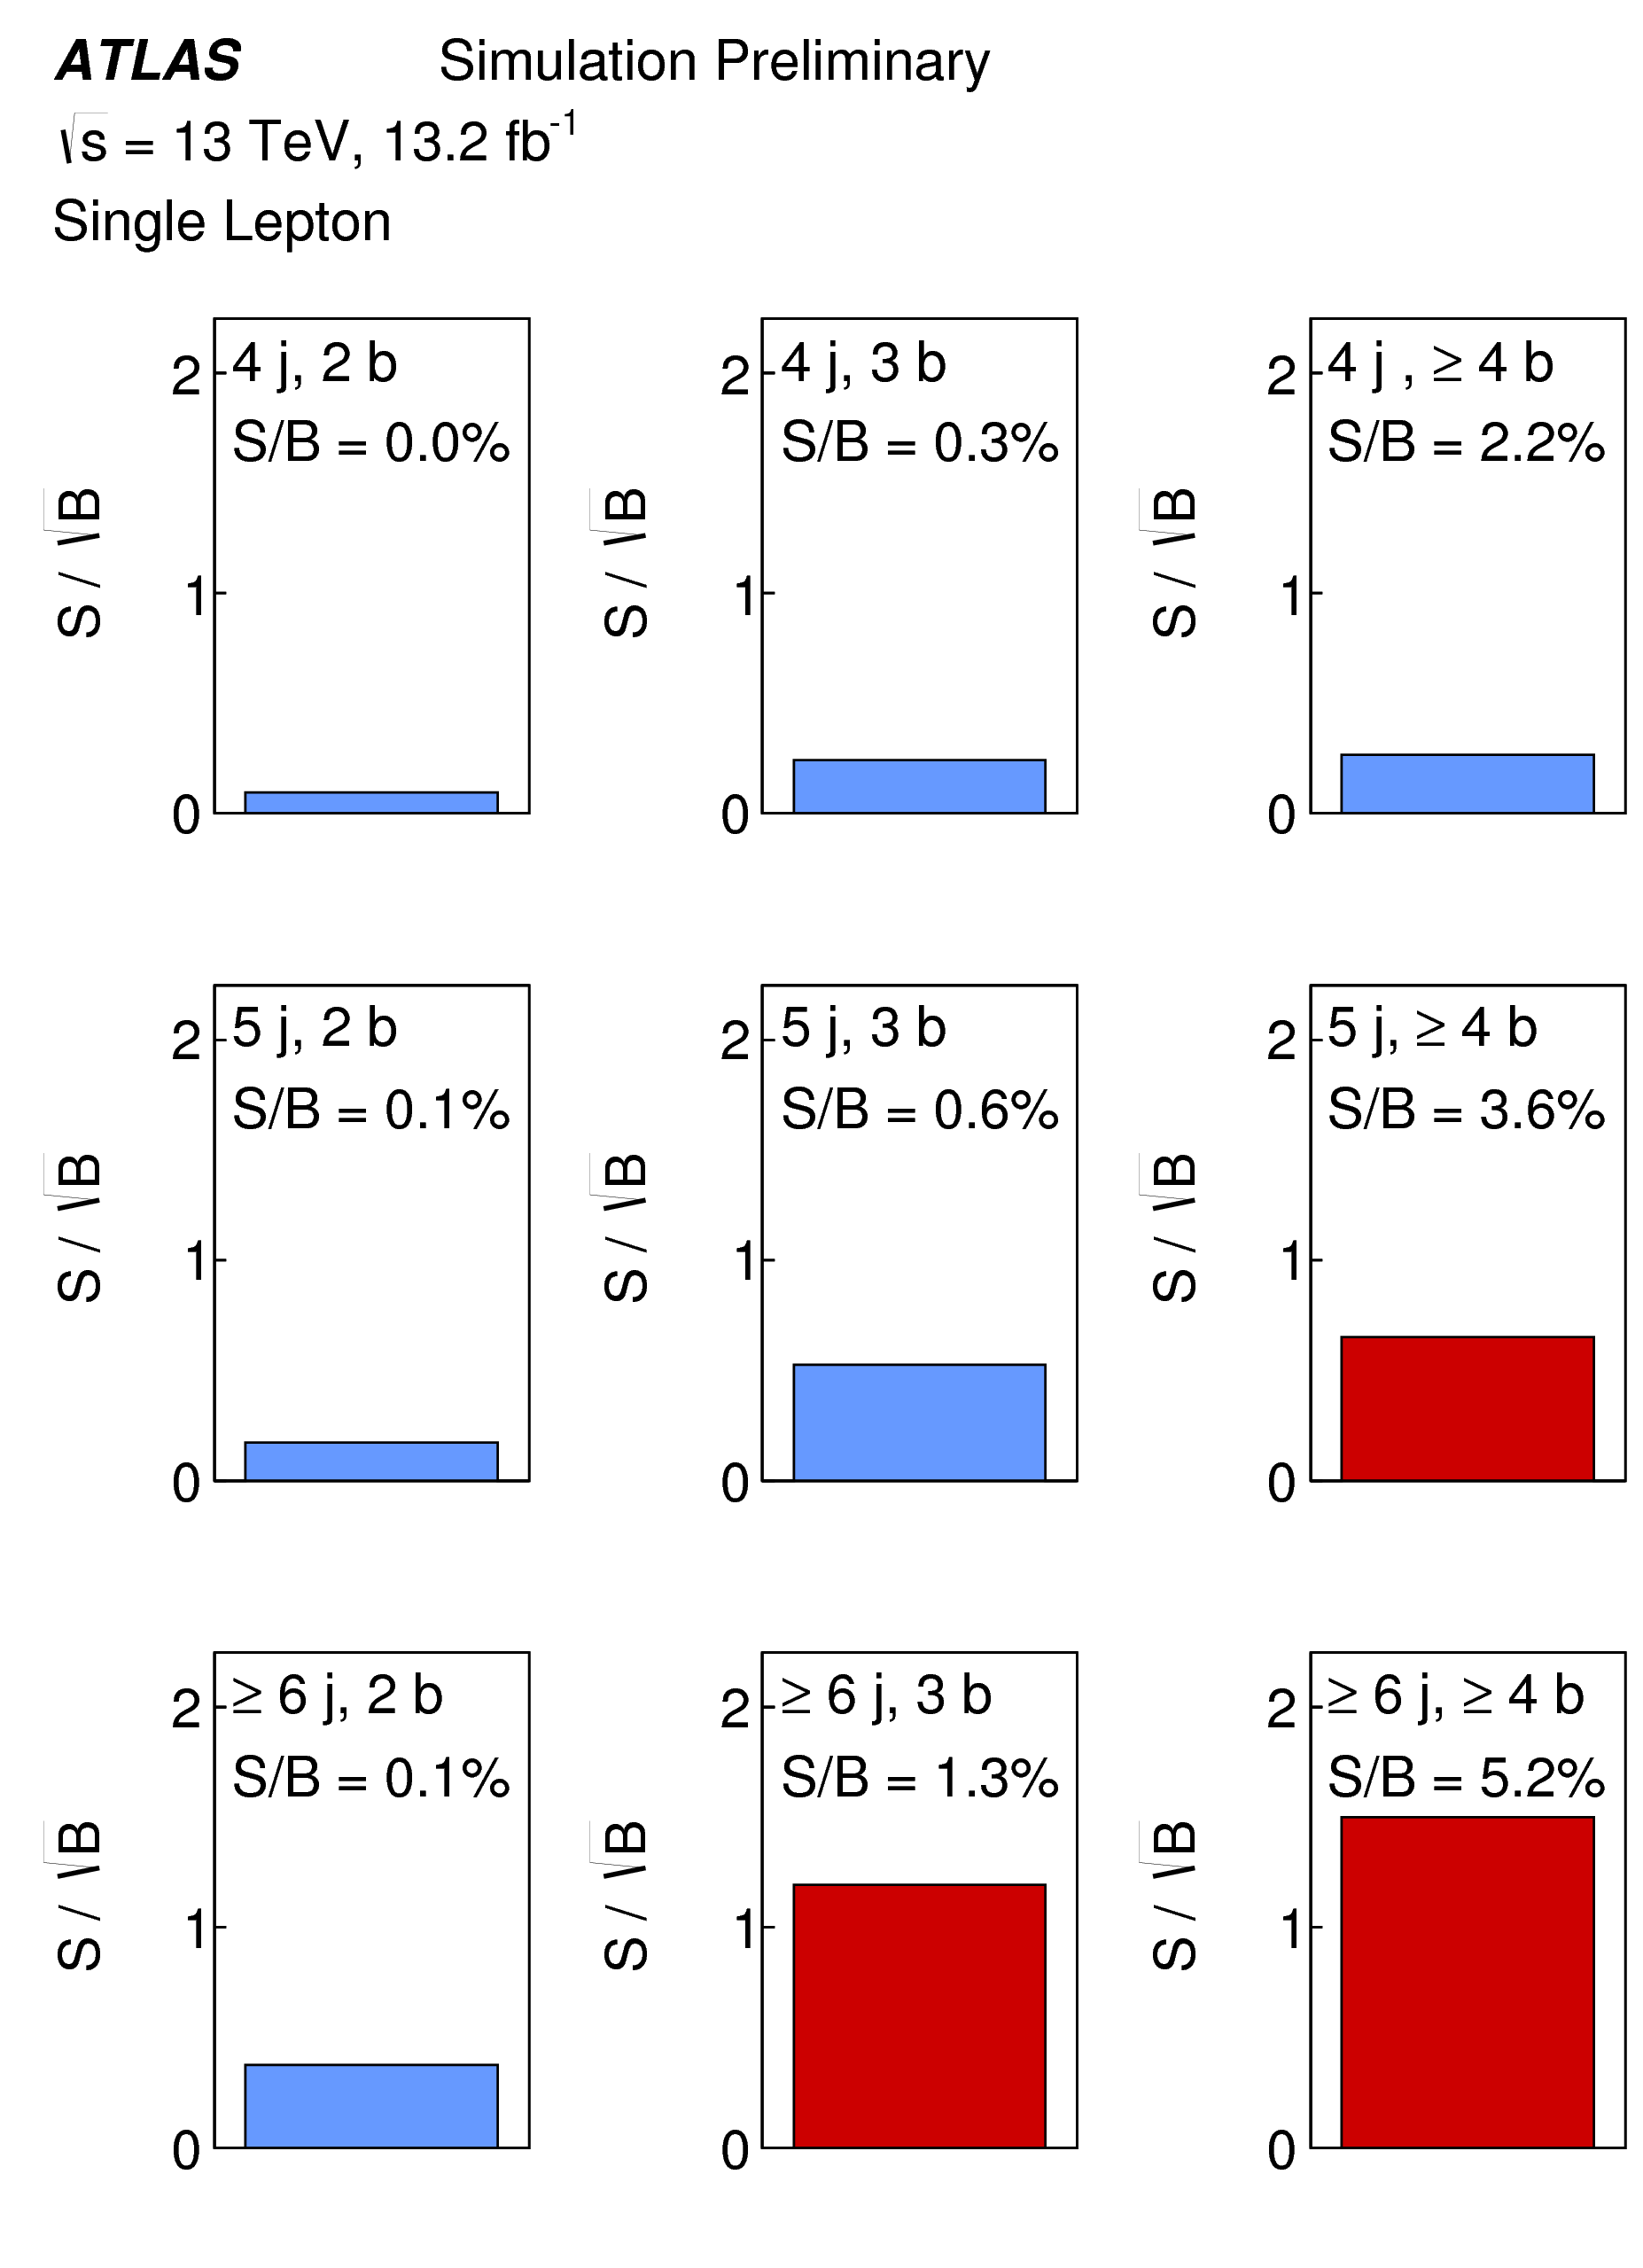
\includegraphics[width=0.9\textwidth]{figures/ttH/fig_03a.png}
  \caption{}
  \label{}
\end{subfigure}
\begin{subfigure}{0.5\textwidth}
  \centering
  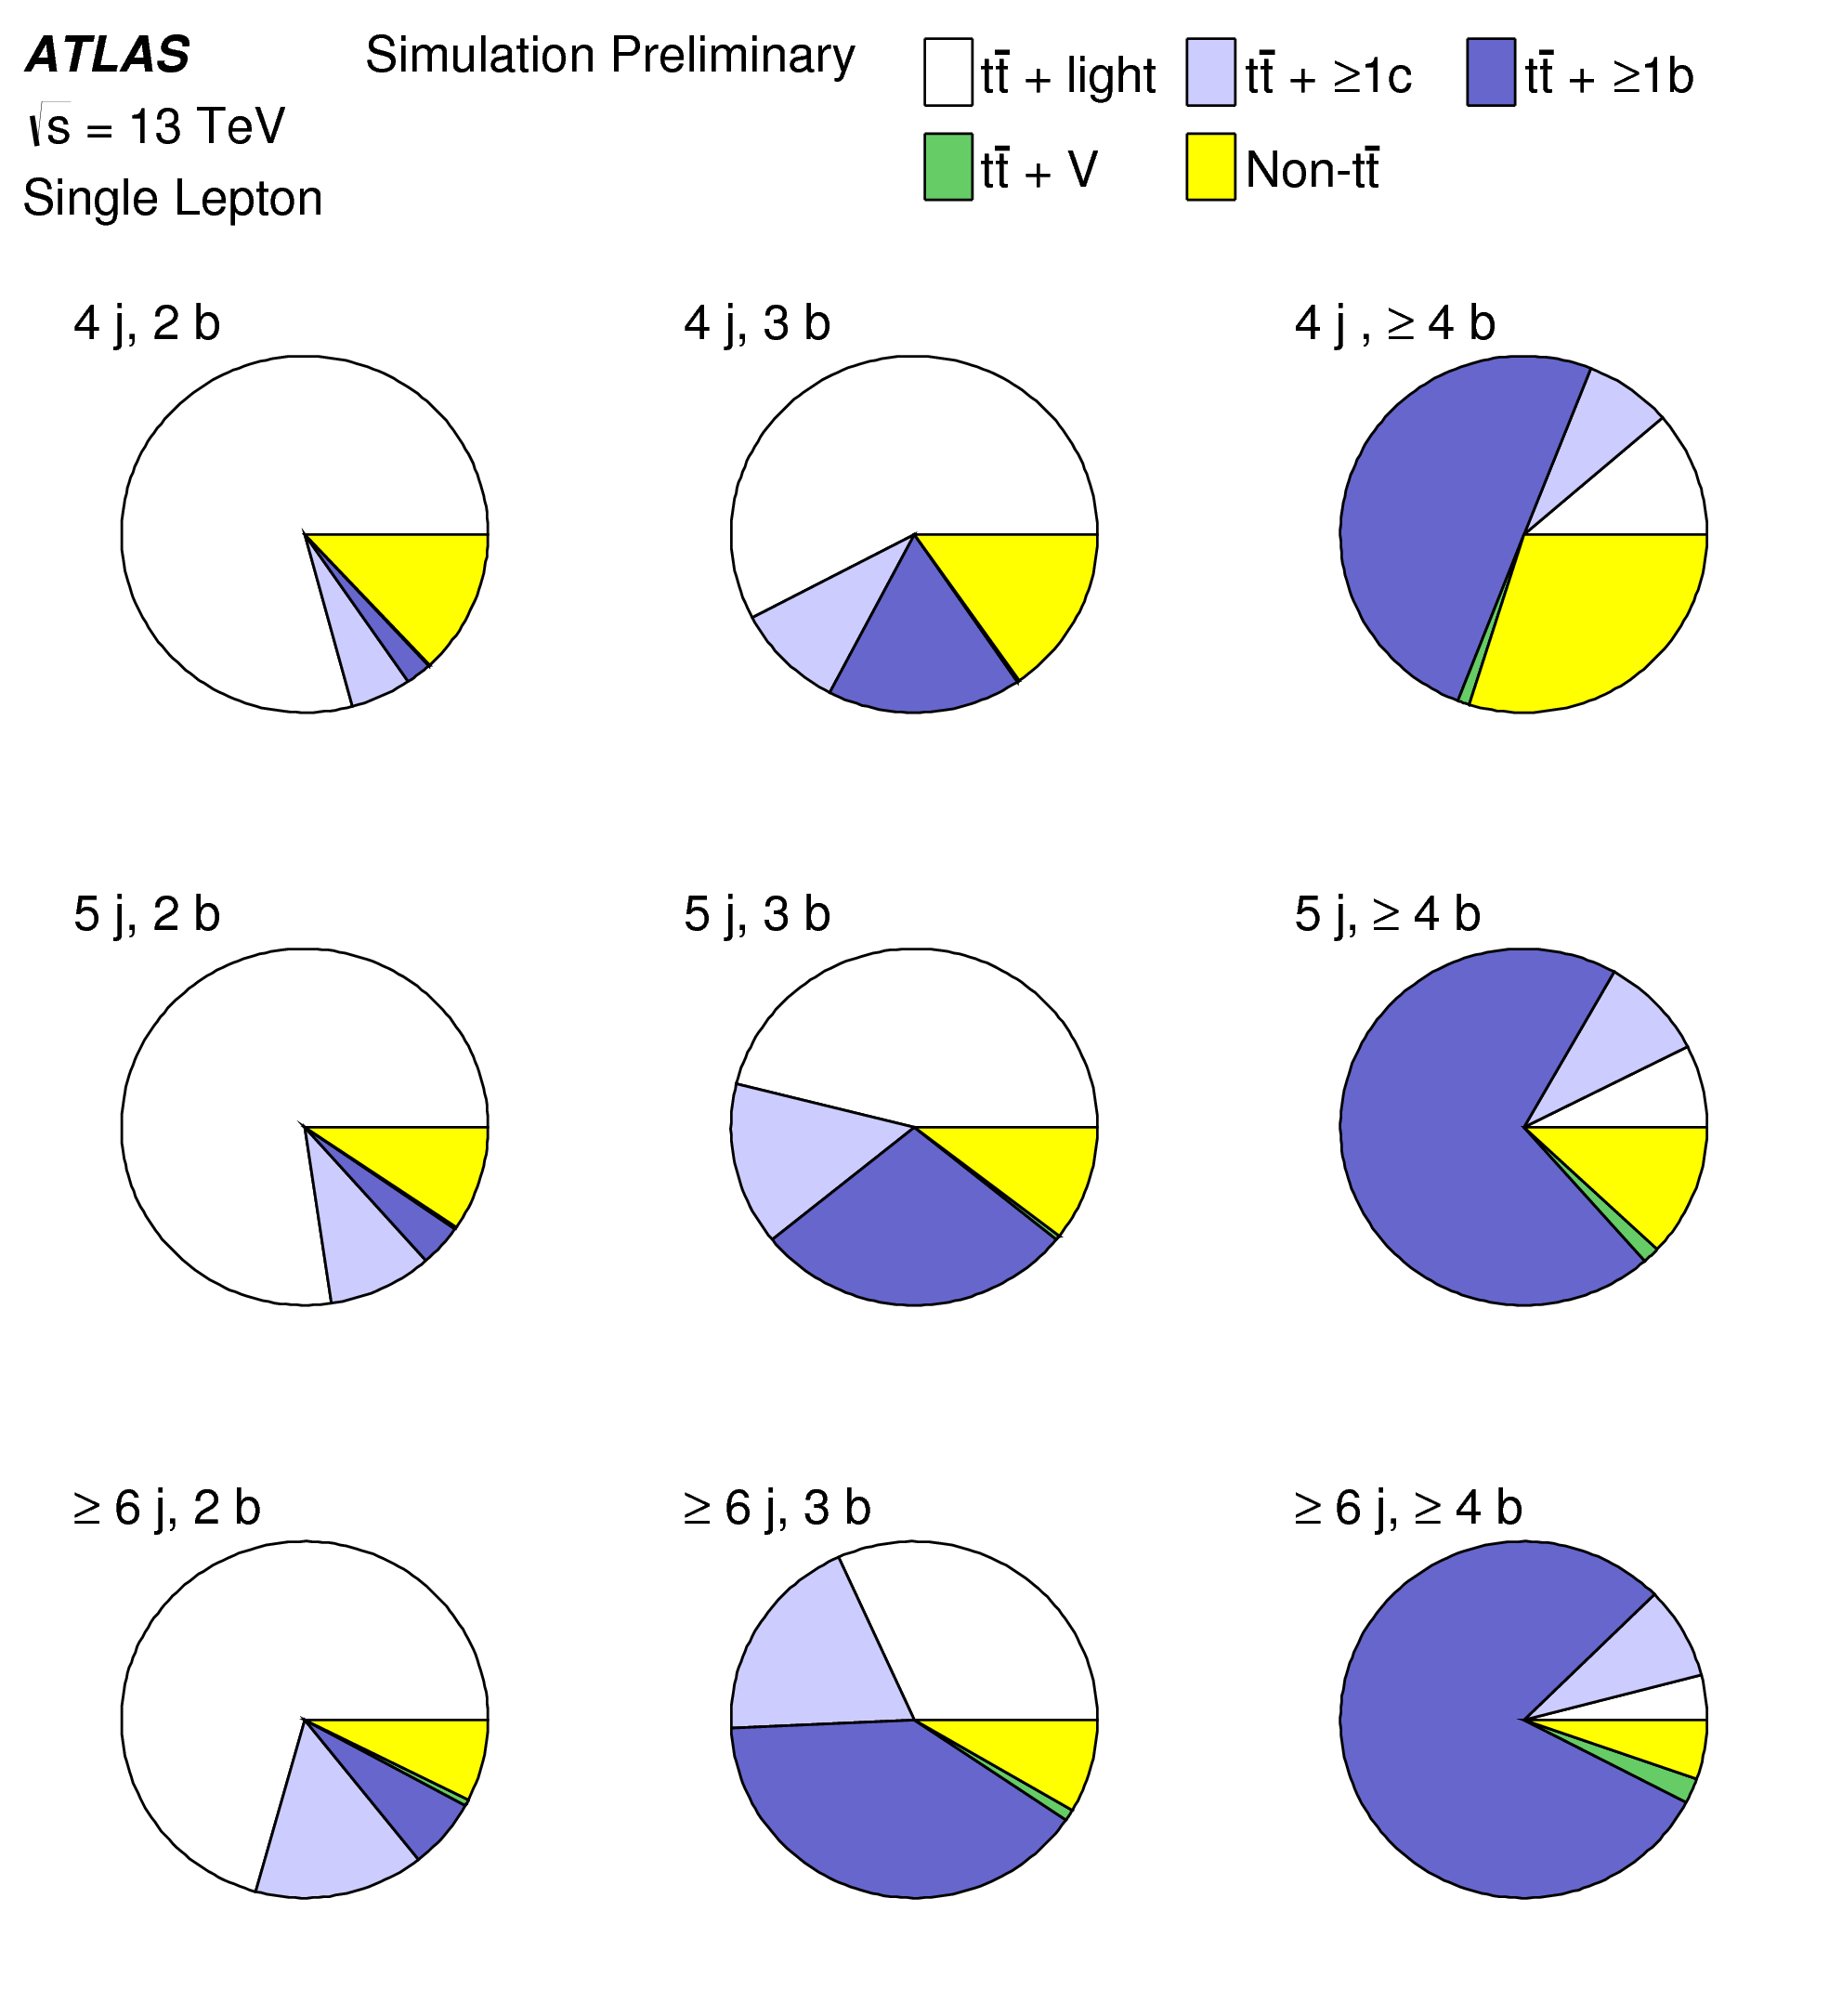
\includegraphics[width=0.9\textwidth]{figures/ttH/fig_03b.png}
  \caption{}
  \label{}
\end{subfigure}

\captionsetup{width=0.85\textwidth}  \caption{\small (a) $S/B$ and $S/\sqrt{B}$ for the analysis regions. Signal regions are shaded in red and control regions in blue. (b) Fractional contribution of the various backgrounds to the total background prediction. The small contributions from single top, $W/Z$+jets, diboson and multijet backgrounds are combined into a single background source referred to as ``Non-$t\bar{t}$''. Each row corresponds to a different jet multiplicity, while each column corresponds to a different $b$-tag multiplicity.}
\label{sec:tth:fig:soverbpie}
\end{figure}